\begin{question}
\noindent An esports tournament designer is creating a symmetric logo for a Valorant-themed banner. Triangle $M$ is rotated to give triangle $M'$, as shown on the grid.

\begin{center}
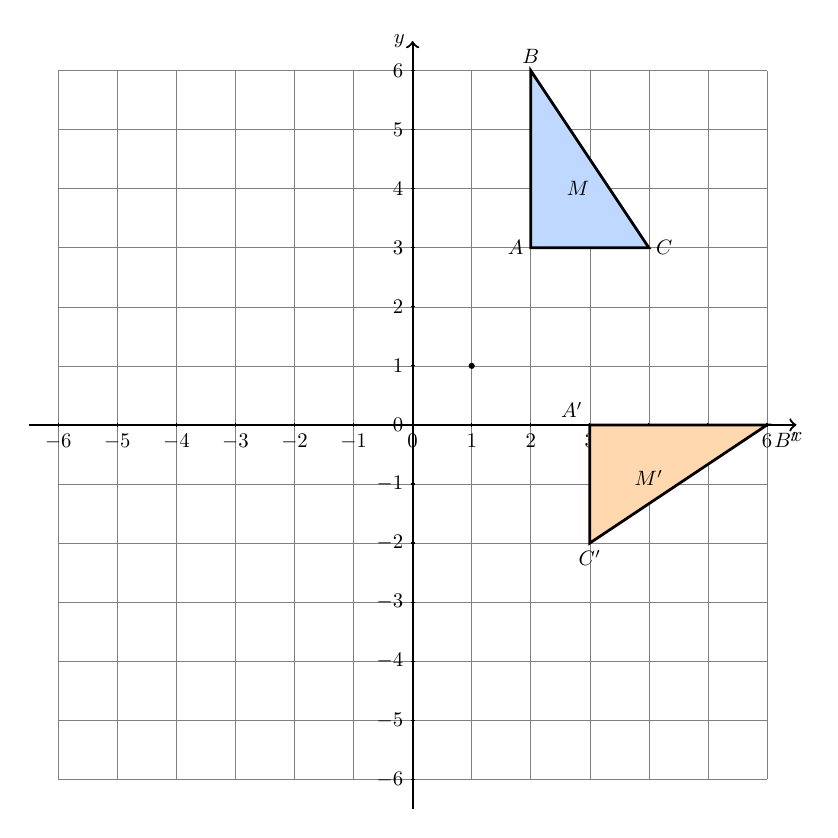
\begin{tikzpicture}[scale=0.75, transform shape]
    \def\axisLimit{6}

    \definecolor{borderColour}{HTML}{000000}
    \definecolor{fillColourM}{HTML}{BFD8FF}
    \definecolor{fillColourMp}{HTML}{FFD8B0}

    % Draw grid
    \draw[step=1cm,gray,very thin] (-\axisLimit,-\axisLimit) grid (\axisLimit,\axisLimit);

    % Draw axes
    \draw[thick,->] (-\axisLimit-0.5,0) -- (\axisLimit+0.5,0) node[anchor=north] {$x$};
    \draw[thick,->] (0,-\axisLimit-0.5) -- (0,\axisLimit+0.5) node[anchor=east] {$y$};

    % Label x-axis and y-axis
    \foreach \x in {-\axisLimit,...,\axisLimit}
        \draw (\x cm,1pt) -- (\x cm,-1pt) node[anchor=north] {$\x$};
    \foreach \y in {-\axisLimit,...,\axisLimit}
        \draw (1pt,\y cm) -- (-1pt,\y cm) node[anchor=east] {$\y$};

    % Triangle M: A(2,3), B(2,6), C(4,3)
    \coordinate (A) at (2,3);
    \coordinate (B) at (2,6);
    \coordinate (C) at (4,3);
    \filldraw[fill=fillColourM, draw=borderColour, line width=1pt] (A) -- (B) -- (C) -- cycle;
    \node[left] at (A) {$A$};
    \node[above] at (B) {$B$};
    \node[right] at (C) {$C$};
    \node at (2.8,4) {$M$};

    % Centre of rotation at (1,1)
    \coordinate (centre) at (1,1);
    \fill[black] (centre) circle (1.5pt);

    % Triangle M': rotate M by 90 degrees clockwise about (1,1)
    % clockwise 90 about (1,1): (x,y) -> (1 + (y-1), 1 - (x-1)) = (y, 2-x)
    % A(2,3) -> (3,0); B(2,6) -> (6,0); C(4,3) -> (3,-2)
    \coordinate (Ap) at (3,0);
    \coordinate (Bp) at (6,0);
    \coordinate (Cp) at (3,-2);
    \filldraw[fill=fillColourMp, draw=borderColour, line width=1pt] (Ap) -- (Bp) -- (Cp) -- cycle;
    \node[above left] at (Ap) {$A'$};
    \node[below right] at (Bp) {$B'$};
    \node[below] at (Cp) {$C'$};
    \node at (4,-0.9) {$M'$};

\end{tikzpicture}
\end{center}

\noindent Describe fully the single transformation that maps triangle $M$ onto triangle $M'$.

\vspace{5cm}

\begin{flushright}
    \answerlines{3}{3}
\end{flushright}
\end{question}
